\section{Test Description and Success Criteria}
This test is located in \texttt{SimCode/dynamics/spacecraftPlus/\_UnitTest/\newline
test\_spacecraftPlus.py}. Depending on the scenario, there are different success criteria. These are outlined in the following subsections:
\subsection{Translation Only with Gravity Scenario}
In this test the simulation is placed into orbit around Earth with point gravity and the spacecraft only has translational equations being evaluated. The following parameters are being tested. 
\begin{itemize}
	\item Conservation of orbital angular momentum
	\item Conservation of orbital energy
	\item Achieving the expected final attitude
\end{itemize}

\subsection{Rotational Only Scenario}
In this test, the spacecraft only has rotational equations being evaluated. The following parameters describe the success criteria.
\begin{itemize}
\item Conservation of rotational angular momentum
\item Conservation of rotational energy
\item Achieving the expected final attitude
\item Switching MRPs check
\end{itemize}

The MRP switching check needs to be discussed. In the simulation the MRPs are switched to the shadow set after one step of the integration adhering to the following equation\cite{schaub}:

\begin{equation}
\begin{gathered}
\begin{aligned}
&\textnormal{\textbf{if}}\quad [s = \vert \bm \sigma(t + dt) \vert ] > 1  \quad \textnormal{\textbf{then}}\\
&\quad \bm \sigma(t + dt) = - \frac{\bm \sigma(t + dt)}{s^2}\\
&\textnormal{\textbf{end if}}
\end{aligned}
\end{gathered}
\label{eq:ballin}
\end{equation}

To check that the switch in the simulation is behaving the way it should, the following check was developed. If the switch happened at time $t_\textnormal{s}$, then there are two variables from the sim that will be used: $\bm \sigma(t_\textnormal{s-1})$ and $\bm \sigma(t_\textnormal{s})$. The intermediate MRP that is switched in the sim is not an output of the simulation, but we will call this variable $\bm \sigma_0(t_\textnormal{s})$. To check the switching the following math occurs: 

\begin{equation}
\bm \sigma_0(t_\textnormal{s}) \approx \bm \sigma(t_\textnormal{s-1}) + \frac{\bm \sigma(t_\textnormal{s-1}) - \bm \sigma(t_\textnormal{s-2})}{\Delta t} \Delta t
\end{equation}
Where this is an Euler approximation to the intermediate MRP before the switch occurs. Now using Eq.~\eqref{eq:ballin} the following definition is made:

\begin{equation}
\bm \sigma_{\textnormal{ch}}(t_\textnormal{s}) = - \frac{\bm \sigma_0(t_\textnormal{s})}{\vert \bm \sigma_0(t_\textnormal{s}) \vert^2}
\end{equation}
Where $\bm \sigma_{\textnormal{ch}}(t_\textnormal{s})$ is the MRP to check vs. the simulation MRP. Therefore, in the integrated test, the test is making sure that $ \bm \sigma(t_\textnormal{s}) \approx \bm \sigma_{\textnormal{ch}}(t_\textnormal{s})$

\subsection{Translational and Rotational Scenario}
In this test, the spacecraft is placed into an orbit with simple gravity and also has rotational states associated with the spacecraft. The following parameters describe the success criteria.
\begin{itemize}
	\item Conservation of orbital angular momentum
	\item Conservation of orbital energy
	\item Achieving the expected final attitude (same as translational only test)
	\item Conservation of rotational angular momentum
	\item Conservation of rotational energy
	\item Achieving the expected final attitude (same as rotational only test)
\end{itemize}

\subsection{Translational BOE Calculation Scenario}

The translational BOE calculation can be seen in Figure~\ref{fig:BOETrans}. In this test a positive force is placed on the hub in the $\hat{\bm b}_1$ direction with no torque and no initial rotation of the spacecraft. This results in the 1 degree of freedom problem seen in Figure~\ref{fig:BOETrans}. The force applied for some length of time, left off for a length of time, and then a negative force is applied ot the system for some length of time. The test is ensuring that Basilisk is giving the same results as the BOE calculation. 

\begin{figure}[htbp]
	\centerline{
		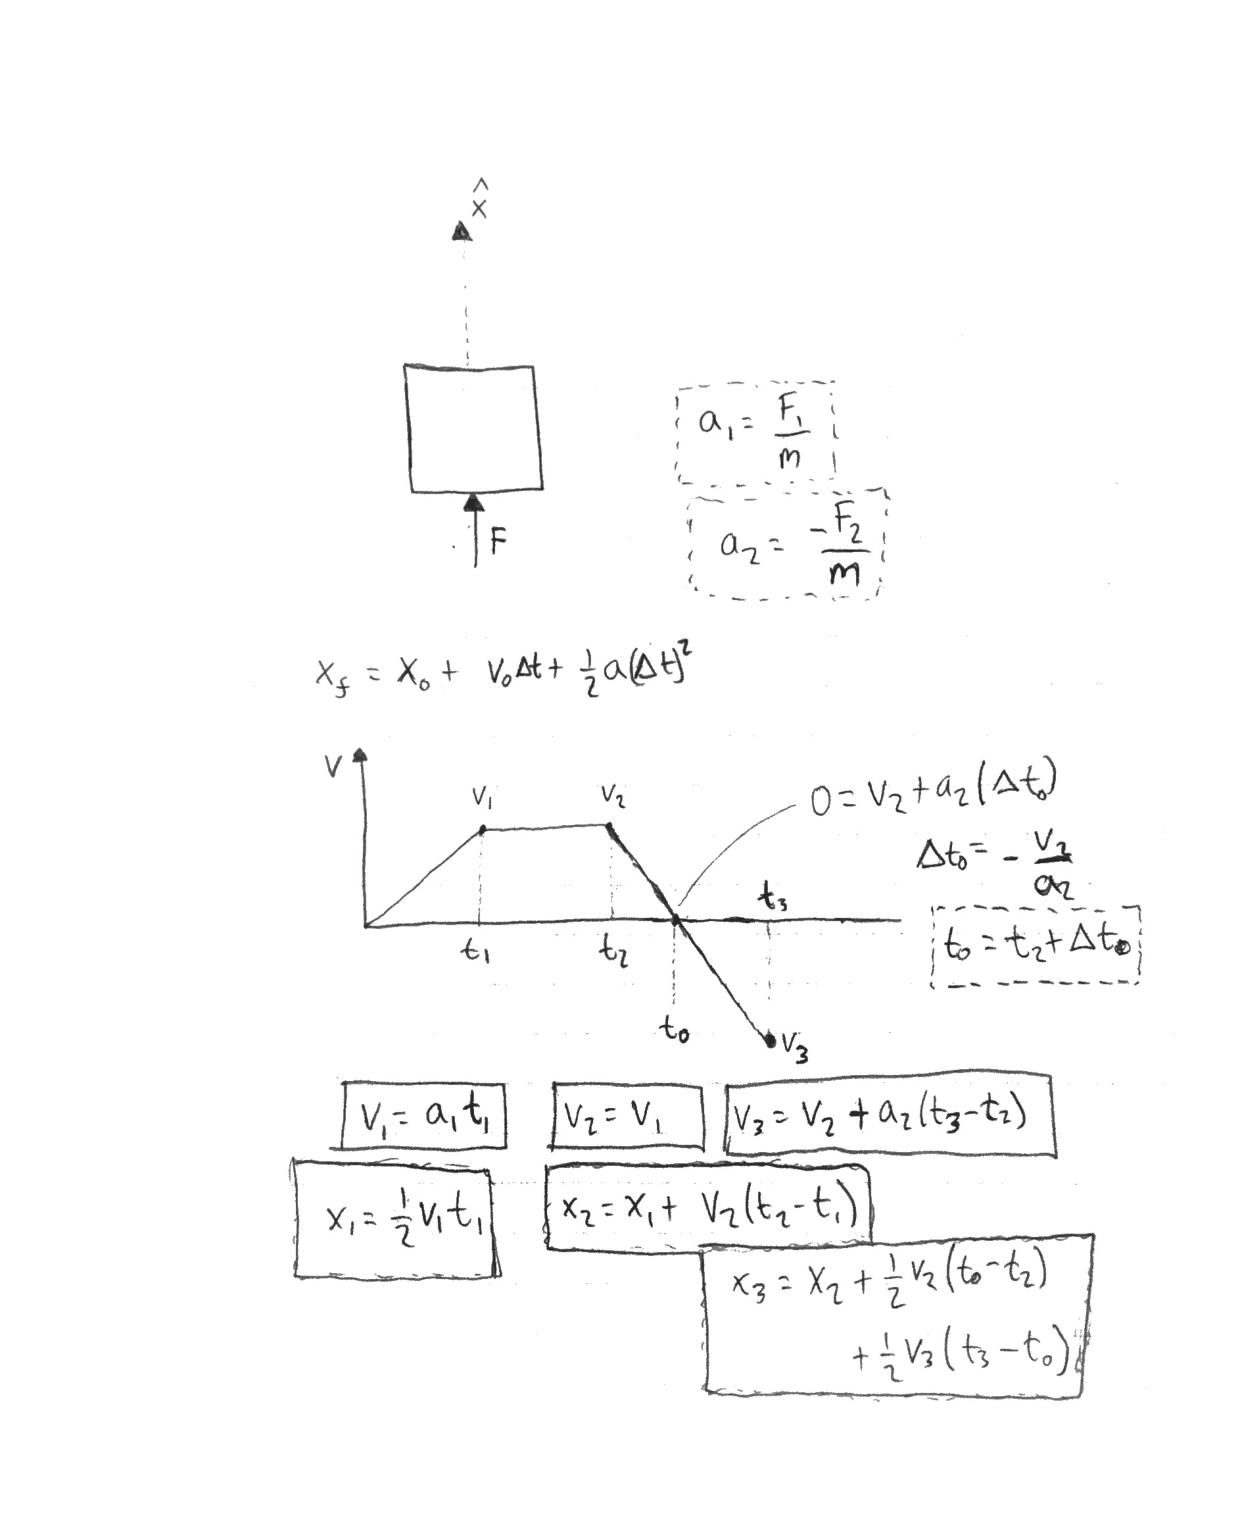
\includegraphics[width=0.8\textwidth]{Figures/TranslationBOE}}
	\caption{Simple Translation BOE Calculation}
	\label{fig:BOETrans}
\end{figure}

\subsection{Rotational BOE Calculation Scenario}

\clearpage

\section{Test Parameters}

Since this is an integrated test, the inputs to the test are the physical parameters of the spacecraft along with the initial conditions of the states. These parameters are outlined in Tables~\ref{tab:hub}-~\ref{tab:initial}. Additionally, the error tolerances can be seen in Table~\ref{tab:errortol}.

\begin{table}[htbp]
	\caption{Spacecraft Hub Parameters}
	\label{tab:hub}
	\centering \fontsize{10}{10}\selectfont
	\begin{tabular}{| c | c | c | c |} % Column formatting, 
		\hline
		\textbf{Name}  & \textbf{Description}  & \textbf{Value} & \textbf{Units} \\
		\hline
		mHub  & mass & 750.0 & kg \\
		\hline
		IHubPntBc\_B & Inertia in $\cal{B}$ frame & $\begin{bmatrix}
		900.0 & 0.0 & 0.0\\
		0.0 & 600.0 & 0.0\\
		0.0 & 0.0 & 600.0
		\end{bmatrix}$ & kg-m$^2$ \\
		\hline
		r\_BcB\_B & CoM Location in $\cal{B}$ frame & $\begin{bmatrix}
		0.0 & 0.0 & 1.0 \end{bmatrix}^T$ & m \\
		\hline
	\end{tabular}
\end{table}

\begin{table}[htbp]
	\caption{Hinged Rigid Body 1 Parameters}
	\label{tab:panel1}
	\centering \fontsize{10}{10}\selectfont
	\begin{tabular}{| c | c | c | c |} % Column formatting, 
		\hline
		\textbf{Name}  & \textbf{Description}  & \textbf{Value} & \textbf{Units} \\
		\hline
		mass  & mass & 100.0 & kg \\
		\hline
		IPntS\_S & Inertia in $\cal{S}$ frame & $\begin{bmatrix}
		100.0 & 0.0 & 0.0\\
		0.0 & 50.0 & 0.0\\
		0.0 & 0.0 & 50.0
		\end{bmatrix}$ & kg-m$^2$ \\
		\hline
		d & CoM location & 1.5 & m \\
		\hline
		k & Spring Constant & 100.0 & N-m/rad \\
		\hline
		c & Damping Term & 0.0 (6.0 - damping scenario) & N-m-s/rad \\
		\hline
		r\_HB\_B & Hinge Location in $\cal{B}$ frame & $\begin{bmatrix}
		0.5 & 0.0 & 1.0 \end{bmatrix}^T$ & m \\
		\hline
		dcm\_HB & $\cal{B}$ to $\cal{H}$ DCM & $\begin{bmatrix}
		-1.0 & 0.0 & 0.0\\
		0.0 & -1.0 & 0.0\\
		0.0 & 0.0 & 1.0
		\end{bmatrix}$ & - \\
		\hline
	\end{tabular}
\end{table}

\begin{table}[htbp]
	\caption{Hinged Rigid Body 2 Parameters}
	\label{tab:panel2}
	\centering \fontsize{10}{10}\selectfont
	\begin{tabular}{| c | c | c | c |} % Column formatting, 
		\hline
		\textbf{Name}  & \textbf{Description}  & \textbf{Value} & \textbf{Units} \\
		\hline
		mass  & mass & 100.0 & kg \\
		\hline
		IPntS\_S & Inertia in $\cal{S}$ frame & $\begin{bmatrix}
		100.0 & 0.0 & 0.0\\
		0.0 & 50.0 & 0.0\\
		0.0 & 0.0 & 50.0
		\end{bmatrix}$ & kg-m$^2$ \\
		\hline
		d & CoM location & 1.5 & m \\
		\hline
		k & Spring Constant & 100.0 & N-m/rad \\
		\hline
		c & Damping Term & 0.0 (7.0 - damping scenario) & N-m-s/rad \\
		\hline
		r\_HB\_B & Hinge Location in $\cal{B}$ frame & $\begin{bmatrix}
		-0.5 & 0.0 & 1.0 \end{bmatrix}^T$ & m \\
		\hline
		dcm\_HB & $\cal{B}$ to $\cal{H}$ DCM & $\begin{bmatrix}
		1.0 & 0.0 & 0.0\\
		0.0 & 1.0 & 0.0\\
		0.0 & 0.0 & 1.0
		\end{bmatrix}$ & - \\
		\hline
	\end{tabular}
\end{table}

\begin{table}[htbp]
	\caption{Initial Conditions for Energy Momentum Conservation Scenarios}
	\label{tab:initial}
	\centering \fontsize{10}{10}\selectfont
	\begin{tabular}{| c | c | c | c |} % Column formatting, 
		\hline
		\textbf{Name}  & \textbf{Description}  & \textbf{Value} & \textbf{Units} \\
		\hline
		(Panel 1) thetaInit  & (Panel 1) Initial $\theta$ & 5.0 & deg \\
		\hline
		(Panel 1) thetaDotInit  & (Panel 1) Initial $\dot{\theta}$ & 0.0 & deg \\
		\hline
		(Panel 2) thetaInit  & (Panel 2) Initial $\theta$ & 0.0 & deg \\
		\hline
		(Panel 2) thetaDotInit  & (Panel 2) Initial $\dot{\theta}$ & 0.0 & deg \\
		\hline
		r\_CN\_NInit & Initial Position of S/C (gravity scenarios) & $\begin{bmatrix}
		-4020339 &	7490567 & 5248299 
		\end{bmatrix}^T$ & m \\
		\hline
		v\_CN\_NInit & Initial Velocity of S/C (gravity scenarios) & $\begin{bmatrix}
		-5199.78 & -3436.68 & 1041.58
		\end{bmatrix}^T$ & m/s \\
		\hline
		r\_CN\_NInit & Initial Position of S/C (no gravity) & $\begin{bmatrix}
		0.1 & -0.4 & 0.3 
		\end{bmatrix}^T$ & m \\
		\hline
		v\_CN\_NInit & Initial Velocity of S/C (no gravity) & $\begin{bmatrix}
		-0.2 & 0.5 & 0.1
		\end{bmatrix}^T$ & m/s \\
		\hline
		sigma\_BNInit & Initial MRP of $\cal{B}$ frame & $\begin{bmatrix}
		0.0 & 0.0 & 0.0
		\end{bmatrix}^T$ & - \\
		\hline
		omega\_BN\_BInit & Initial Angular Velocity of $\cal{B}$ frame & $\begin{bmatrix}
		0.1 & -0.1 & 0.1
		\end{bmatrix}^T$ & rad/s \\
		\hline
	\end{tabular}
\end{table}

\begin{table}[htbp]
	\caption{Error Tolerance - Note: Relative Tolerance is $\textnormal{abs}(\frac{\textnormal{truth} - \textnormal{value}}{\textnormal{truth}}$)}
	\label{tab:errortol}
	\centering \fontsize{10}{10}\selectfont
	\begin{tabular}{| c | c |} % Column formatting, 
		\hline
		Test   & Relative Tolerance \\
		\hline
		Energy and Momentum Conservation & 1e-10 \\
		\hline
		Steady State Deflection & 1e-6 \\
		\hline
		Frequency verification & 5e-3 \\
		\hline
		Max deflection with force on & 5e-3 \\
		\hline
		Max deflection with force off & 5e-3 \\
		\hline
		Lagrangian vs Basilisk comparison & 1e-10 \\
		\hline	
	\end{tabular}
\end{table}

\clearpage

\section{Test Results}

\subsection{Translation Only with Gravity Scenario}
\input{AutoTex/ChangeInOrbitalEnergyTranslationOnly}
\input{AutoTex/ChangeInOrbitalAngularMomentumTranslationOnly}
\clearpage

\subsection{Rotational Only Scenario}
\input{AutoTex/ChangeInRotationalEnergyRotationOnly}
\input{AutoTex/ChangeInRotationalAngularMomentumRotationOnly}
\input{AutoTex/MRPs}
\input{AutoTex/MRPSwitching}
\clearpage

\subsection{Translational and Rotational Scenario}
\input{AutoTex/ChangeInOrbitalEnergyTranslationAndRotation}
\input{AutoTex/ChangeInOrbitalAngularMomentumTranslationAndRotation}
\input{AutoTex/ChangeInRotationalEnergyTranslationAndRotation}
\input{AutoTex/ChangeInRotationalAngularMomentumTranslationAndRotation}
\clearpage

\subsection{Translational BOE Calculation Scenario}
\input{AutoTex/TranslationPositionBOE}
\input{AutoTex/TranslationVelocityBOE}
\clearpage

\subsection{Rotational BOE Calculation Scenario}

\clearpage
